%
% Diplomarbeit mit LaTeX
% ===========================================================================
% This is part of the book "Diplomarbeit mit LaTeX".
% Copyright (c) 2002-2005 Tobias Erbsland, Andreas Nitsch
% See the file diplomarbeit_mit_latex.tex for copying conditions.
%

\chapter{Installation}
\label{sec:installation}
\index{Installation|(}

\section{MiKTeX}
\index{Installation!MiKTeX|(}

Mit \enquote{MiKTeX}~\cite{MiKTeX} existiert neben \enquote{Tex Live} eine weitere \DMLLaTeX"=Distribution, die mittlerweile für Windows, macOS und Linux verfügbar ist und sich einfach installieren lässt.
MiKTeX ist freie Software, d.\,h. ist kostenlos und wird unter einer Open-Source-Lizenz vertrieben.

Im Folgenden wird die Installation unter Windows beschrieben. Für andere Systeme werden Tutorials auf der MiKTeX-Website angeboten. Insbesondere für Linux bietet sich stattdessen die Installation von Tex Live an, was sich in der Regel mit einer Zeile erledigen lässt.

\subsection{Herunterladen des Setup-Programms}

Unter 
\urlindent{https://www.miktex.org/}
findest du verschiedene Versionen des Installers, welche du herunterladen kannst.

Empfehlenswert ist hier der \enquote{Basic MiKTeX Installer}, da er die besonders häufig verwendeten Pakete bereits enthält, sodass diese nicht mehr nachträglich heruntergeladen werden müssen. Diese Installer-Datei ist einige Hundert MB groß.

Wähle diesen Link an und lade den Installer herunter.

\subsection{Starten des Setups}
Der im Folgenden dargestellte Ablauf der Installation mag sich im Laufe der Zeit geringfügig ändern. Die jeweils aktuellsten Informationen befinden sich (allerdings nur auf Englisch) unter
\urlindent[.]{https://miktex.org/howto/install-miktex}

\begin{figure}[hb]
	\begin{captionbeside}{Nach dem Start des Programms erscheint dieser Screen. Du musst die Lizenzbedingungen akzeptieren.}[l]
		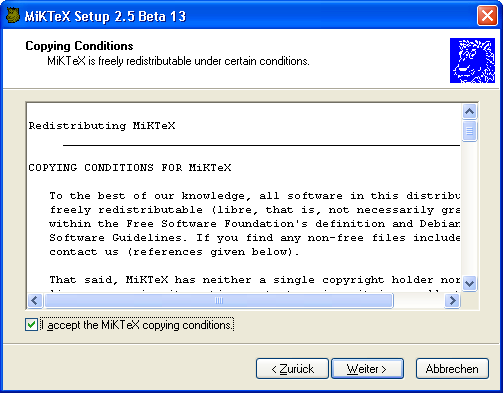
\includegraphics[width=7cm]{images/MiKTeX-install-01.png}
	\end{captionbeside}
	\label{fig:install01}
\end{figure}

\begin{figure}[hb]
	\begin{captionbeside}[Auswahl des Installationsmodus]{Wähle hier, ob nur Dein aktueller Nutzer oder alle am PC angemeldeten Nutzer MiKTeX nutzen können sollen. Letzteres ist empfehlenswert, damit es keine Probleme gibt.}[l]
		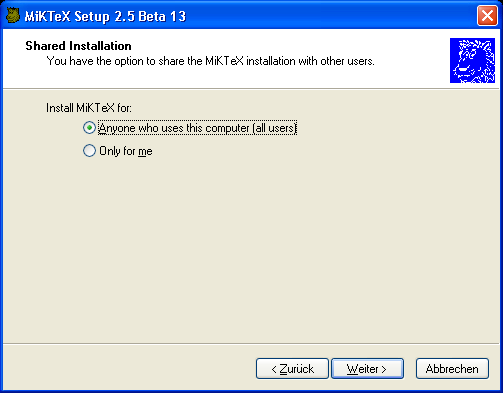
\includegraphics[width=7cm]{images/MiKTeX-install-02.png}
	\end{captionbeside}
	\label{fig:install02}
\end{figure}

\begin{figure}[hb]
	\begin{captionbeside}[Ziel der Installation wählen]{Hier kann das Ziel der Installation gewählt werden.}[l]
		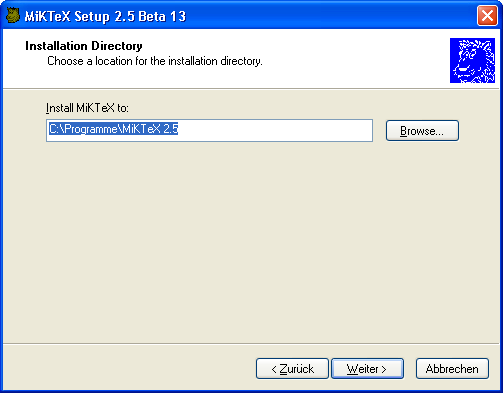
\includegraphics[width=7cm]{images/MiKTeX-install-03.png}
	\end{captionbeside}
	\label{fig:install03}
\end{figure}

\begin{figure}[hb]
	\begin{captionbeside}[Bevorzugtes Papierformat]{Für den deutschen Sprachraum ist A4 ein sinnvoller Standard. Da Du für einzelne Dokumente das jeweilige Papierformat bestimmen kannst, gilt diese Einstellung nur für Dokumente ohne weitere Angabe.}[l]
		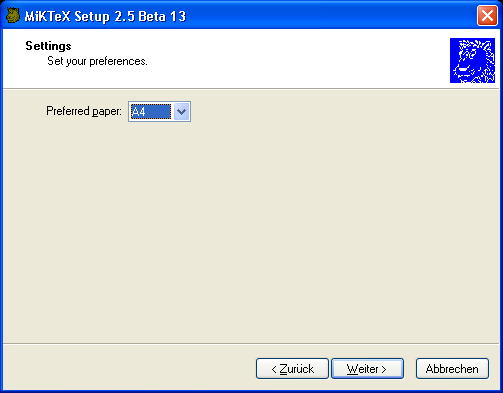
\includegraphics[width=7cm]{images/MiKTeX-install-04.png}
	\end{captionbeside}
	\label{fig:install04}
\end{figure}

\begin{figure}[th]
	\begin{captionbeside}{Der Bestätigungsscreen vor dem Start der eigentlichen Installation.}[l]
		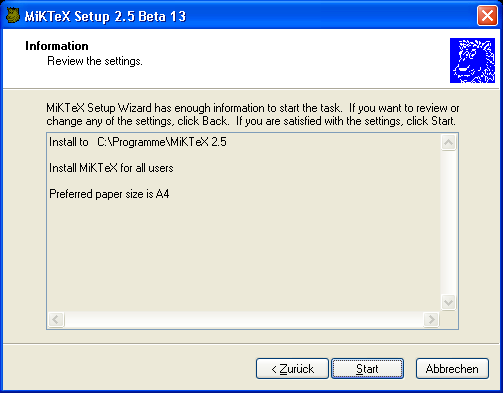
\includegraphics[width=7cm]{images/MiKTeX-install-05.png}
	\end{captionbeside}
	\label{fig:install06}
\end{figure}

\begin{figure}[th]
	\begin{captionbeside}[Die Pakete werden installiert]{Nun werden die einzelnen Pakete installiert.}[l]
		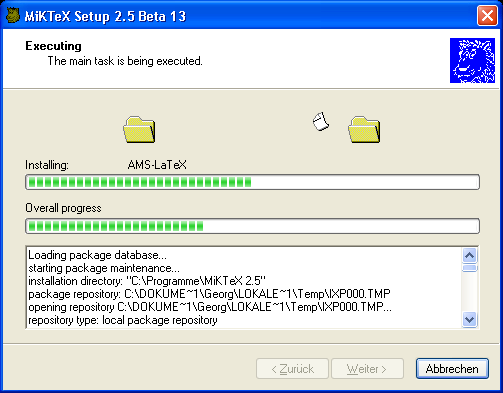
\includegraphics[width=7cm]{images/MiKTeX-install-07.png}
	\end{captionbeside}
	\label{fig:install07}
\end{figure}

\begin{figure}[th]
	\begin{captionbeside}[Das Ende des Setups]{Jetzt folgt noch ein kurzer Bestätigungsscreen und nach einem Klick auf \enquote{Close} wird das Setup beendet.}[l]
		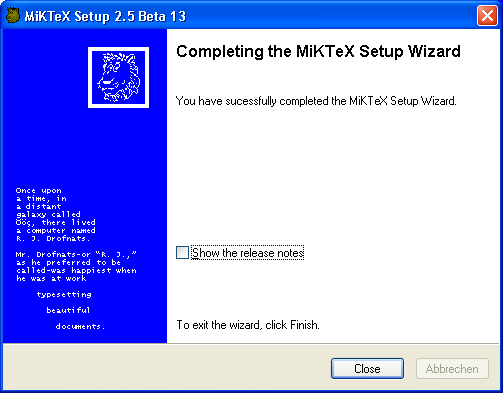
\includegraphics[width=7cm]{images/MiKTeX-install-08.png}
	\end{captionbeside}
	\label{fig:install08}
\end{figure}

\clearpage % Warten bis alle Floats ausgegeben sind.

\subsection{Herunterladen der Pakete}
\label{subsec:instpakete}

Während der Benutzung von MiKTeX und TeXnicCenter wirst Du bei fehlenden Paketen gefragt, ob sie heruntergeladen werden sollen. Dies ist ein bequemer und minimalistischer Ansatz, da nur genau die Pakete installiert werden, die Du tatsächlich brauchst, und diese immer in der aktuellen Version aus dem Netz geladen werden. 

Alternativ Du kannst alle verfügbaren Pakete auf einmal herunterladen. Das ist z.\,B. dann sinnvoll, wenn Du nur vorübergehend breitbandig mit dem Internet verbunden bist und Festplattenplatz keinen Engpass darstellt (die allermeisten Pakete wirst Du nie verwenden, also den davon eingenommenen Platz verschwenden). Auf diese Weise stehen immer alle Pakete zur Verfügung.

Wie du manuell einige oder alle Pakete installieren kannst, ist in den Abbildungen \ref{fig:install10} bis \ref{fig:install05b} beschrieben. 

\begin{figure}[hb]
	\begin{captionbeside}[MiKTeX Package Manager starten]{Rufe Start -- Programme -- MiKTeX -- Browse Packages auf. Der \enquote{MiKTeX Package Manager} wird gestartet. Du wählst die gewünschten Pakete aus, indem Du die Steuerung-Tastste gedrückt hälst und mit der Maus auf einzelne Pakete klickst, um mehrere verstreute zu markieren, bzw. indem Du die Umschalt-Tastste gedrückt hälst, um mehrere benachbarte Blöcke auszuwählen.)}[l]
		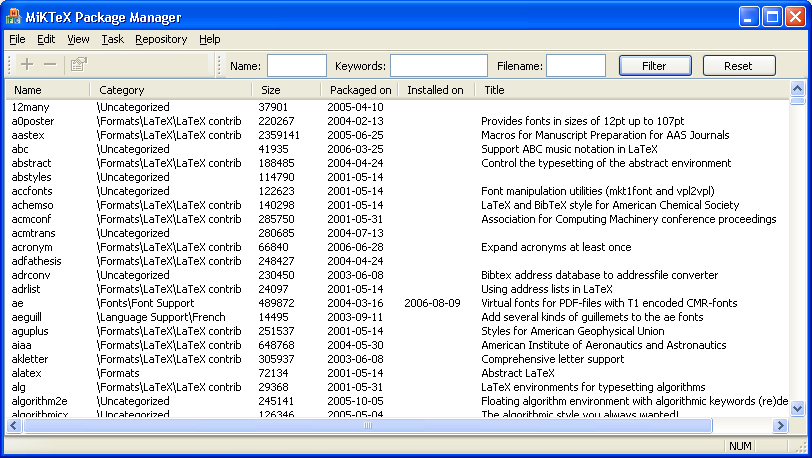
\includegraphics[width=7cm]{images/MiKTeX-packet-install-01.png}
	\end{captionbeside}
	\label{fig:install10}
\end{figure}

\begin{figure}[hb]
	\begin{captionbeside}[Auswahl der Pakete und Start der Installation]{Hast Du die gewünschten Pakete ausgewählt, klickst Du auf das Plus-Icon bzw. gehst im Menü auf Task -- Install. Dieser Informationsbildschirm erscheint, den Du mit OK bestätigst.}[l]
		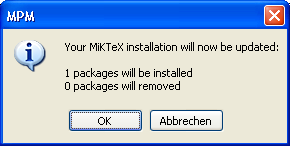
\includegraphics[width=7cm]{images/MiKTeX-packet-install-02.png}
	\end{captionbeside}
	\label{fig:install03b}
\end{figure}

\begin{figure}
	\begin{captionbeside}[Download]{Während die Pakete aus dem Netz geladen werden, werden Dir Statusinformationen angezeigt. Klicke danach auf Close. Damit ist die Paketinstallation beendet.}[l]
		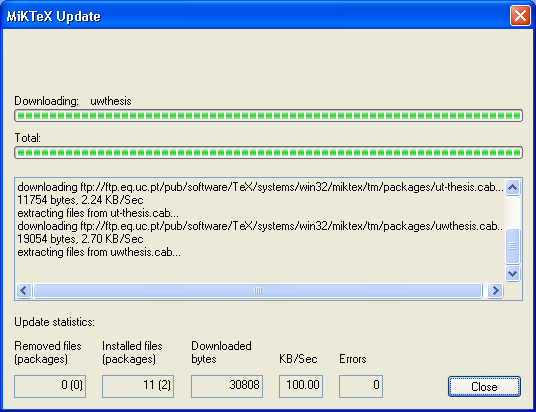
\includegraphics[width=7cm]{images/MiKTeX-packet-install-03.png}
	\end{captionbeside}
	\label{fig:install05b}
\end{figure}

\index{Installation!MiKTeX|)}

\clearpage % Warten bis alle Floats ausgegeben sind.

\section{Der Editor TeXnicCenter}
\index{Installation!TeXnicCenter|(}

Um \DMLLaTeX"=Dokumente einfach editieren zu können, bietet sich unter Windows der freie Editor \enquote{TeXnicCenter}~\cite{TeXnicCenter} an. Dieser unterstützt einfache Navigation in der Dokumentstruktur, Projektverwaltung und einfachen Aufruf von \DMLLaTeX.

Alternativen dazu sind die TeX-Editoren \enquote{Kile} und \enquote{Texmaker}, die auch für Linux erhältlich sind; letzterer auch für macOS.

\subsection{Herunterladen von TeXnicCenter}

Auf der TeXnicCenter"=Webseite
\urlindent{https://www.texniccenter.org/}
wählst du in der Navigation \enquote{Download} an und in der folgenden Liste \enquote{TeXnicCenter 2.02 Stable (64 Bit)} aus. Die 32-Bit-Variante ist nur für sehr alte Computer gedacht. Möglicherweise ist mittlerweile auch eine neuere Version erschienen.

\subsection{Starten des Setups}

Starte das heruntergeladene Setup. Die Installation ist in den Abbildungen \ref{fig:install20} bis \ref{fig:install27} beschrieben.

\begin{figure}[hb]
	\begin{captionbeside}[Startscreen des Installationsassistenten]{Es erscheint der Installationsassistent.}[l]
		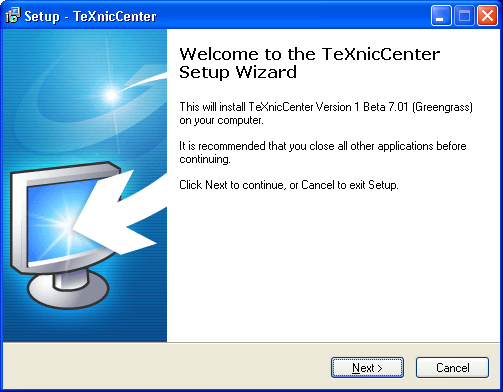
\includegraphics[width=7cm]{images/TeXnicCenter-install-01.png}
	\end{captionbeside}
	\label{fig:install20}
\end{figure}

\begin{figure}[hb]
	\begin{captionbeside}[Anzeige der GPL]{Die GNU General Public License~\cite{GPL} muss akzeptiert werden.}[l]
		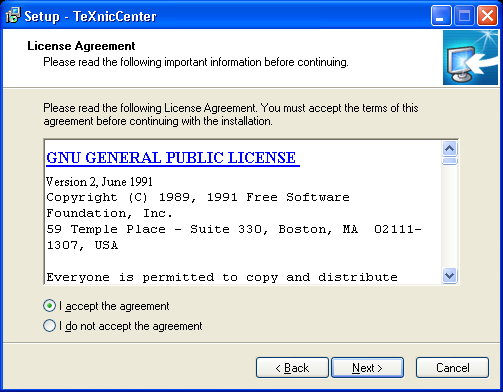
\includegraphics[width=7cm]{images/TeXnicCenter-install-02.png}
	\end{captionbeside}
	\label{fig:install21}
\end{figure}

\begin{figure}[hb]
	\begin{captionbeside}[Wahl des Installationsverzeichnisses]{Hier wählst du das Verzeichnis aus, in das der Editor installiert werden soll. Am besten übernimmst du die Vorgabe.}[l]
		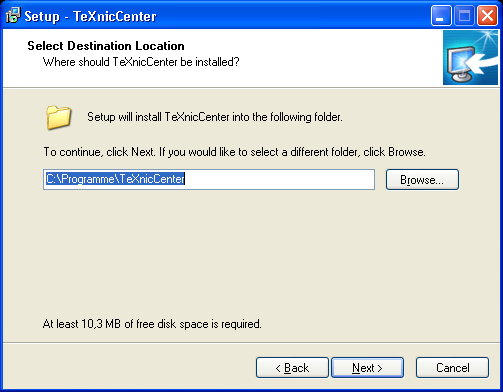
\includegraphics[width=7cm]{images/TeXnicCenter-install-03.png}
	\end{captionbeside}
	\label{fig:install22}
\end{figure}

\begin{figure}[hb]
	\begin{captionbeside}[Frage nach der Installationsart]{Jetzt wirst du nach der Installationsart gefragt. Hier wählst du \enquote{Typical} aus.}[l]
		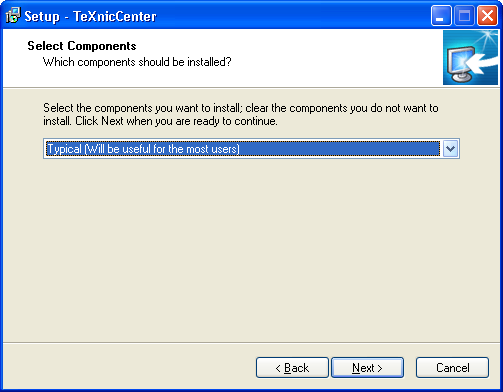
\includegraphics[width=7cm]{images/TeXnicCenter-install-04.png}
	\end{captionbeside}
	\label{fig:install23}
\end{figure}

\begin{figure}[hb]
	\begin{captionbeside}[Wahl des Namens im Startmenü]{Auch bei der Frage nach dem Namen des Startmenüeintrags kannst du die Voreinstellung übernehmen.}[l]
		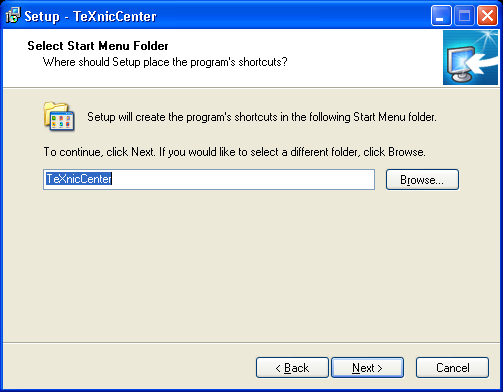
\includegraphics[width=7cm]{images/TeXnicCenter-install-05.png}
	\end{captionbeside}
	\label{fig:install24}
\end{figure}

\begin{figure}[thb]
	\begin{captionbeside}[Frage, ob ein Icon auf dem Desktop erzeugt werden soll]{Je nach Wunsch kannst du hier ein Icon auf dem Desktop und/oder einen Eintrag in das \enquote{Senden an} Kontextmenü erzeugen lassen.}[l]
		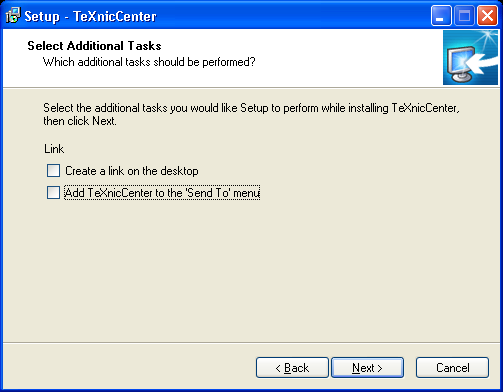
\includegraphics[width=7cm]{images/TeXnicCenter-install-06.png}
	\end{captionbeside}
	\label{fig:install25}
\end{figure}

\begin{figure}[thb]
	\begin{captionbeside}[Eine Zusammenfassung der Installation]{Jetzt folgt noch eine Zusammenfassung der Installationsangaben.}[l]
		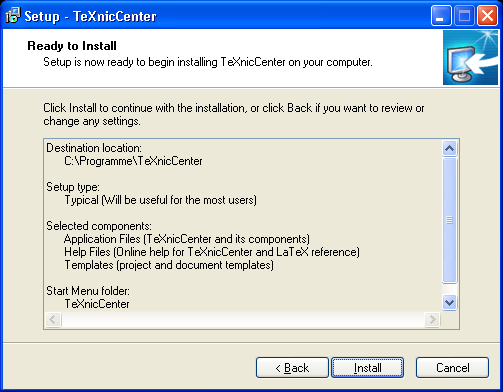
\includegraphics[width=7cm]{images/TeXnicCenter-install-07.png}
	\end{captionbeside}
	\label{fig:install26}
\end{figure}

\begin{figure}[thb]
	\begin{captionbeside}[TeXnicCenter ist installiert]{Schließlich wurde TeXnicCenter erfolgreich installiert.}[l]
		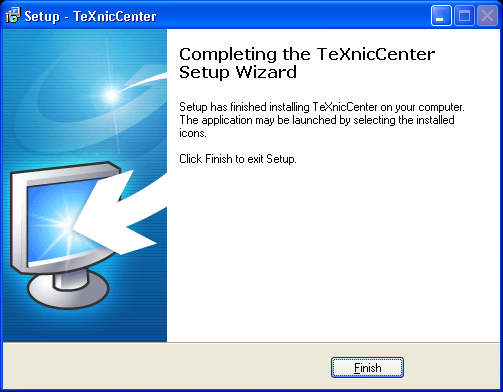
\includegraphics[width=7cm]{images/TeXnicCenter-install-08.png}
	\end{captionbeside}
	\label{fig:install27}
\end{figure}

\index{Installation!TeXnicCenter|)}

\clearpage % Warten bis alle Floats ausgegeben sind.


\section{PDF-Viewer}
\index{Installation!Adobe Reader}

Zur Betrachtung der von uns mittels \DMLLaTeX{} erzeugten PDF-Dateien eignen sich alle gängigen PDF-Viewer. Unter Windows ist der proprietäre \enquote{Adobe Acrobat Reader} vermutlich der verbreitetste. Daneben gibt es freie Betrachter wie \enquote{Evince} oder \enquote{Okular}, die unter allen drei großen Betriebssystemen laufen. 

Mittlerweile können auch Webbrowser wie Firefox oder Chrome bzw. Chromium PDF-Dateien anzeigen, weshalb auf eine Installationsanleitung in dieser Stelle verzichtet wird.

\index{Installation|)}
